\documentclass[12pt]{article}
\setlength{\parskip}{2pt}%
\setlength{\parindent}{0pt}%
\usepackage{enumitem, amsmath, graphicx, wrapfig, float, nccmath, verbatim, fancyvrb, geometry, changepage}
\usepackage[export]{adjustbox}
\title{%
   ECE-471 Selected Topics in Machine Learning \\
   Prof. Curro \\
   Assignment 2}
\author{Evan Bubniak}
\begin{document}
\maketitle

\section{Results}

\begin{figure}[H]
   \centering
   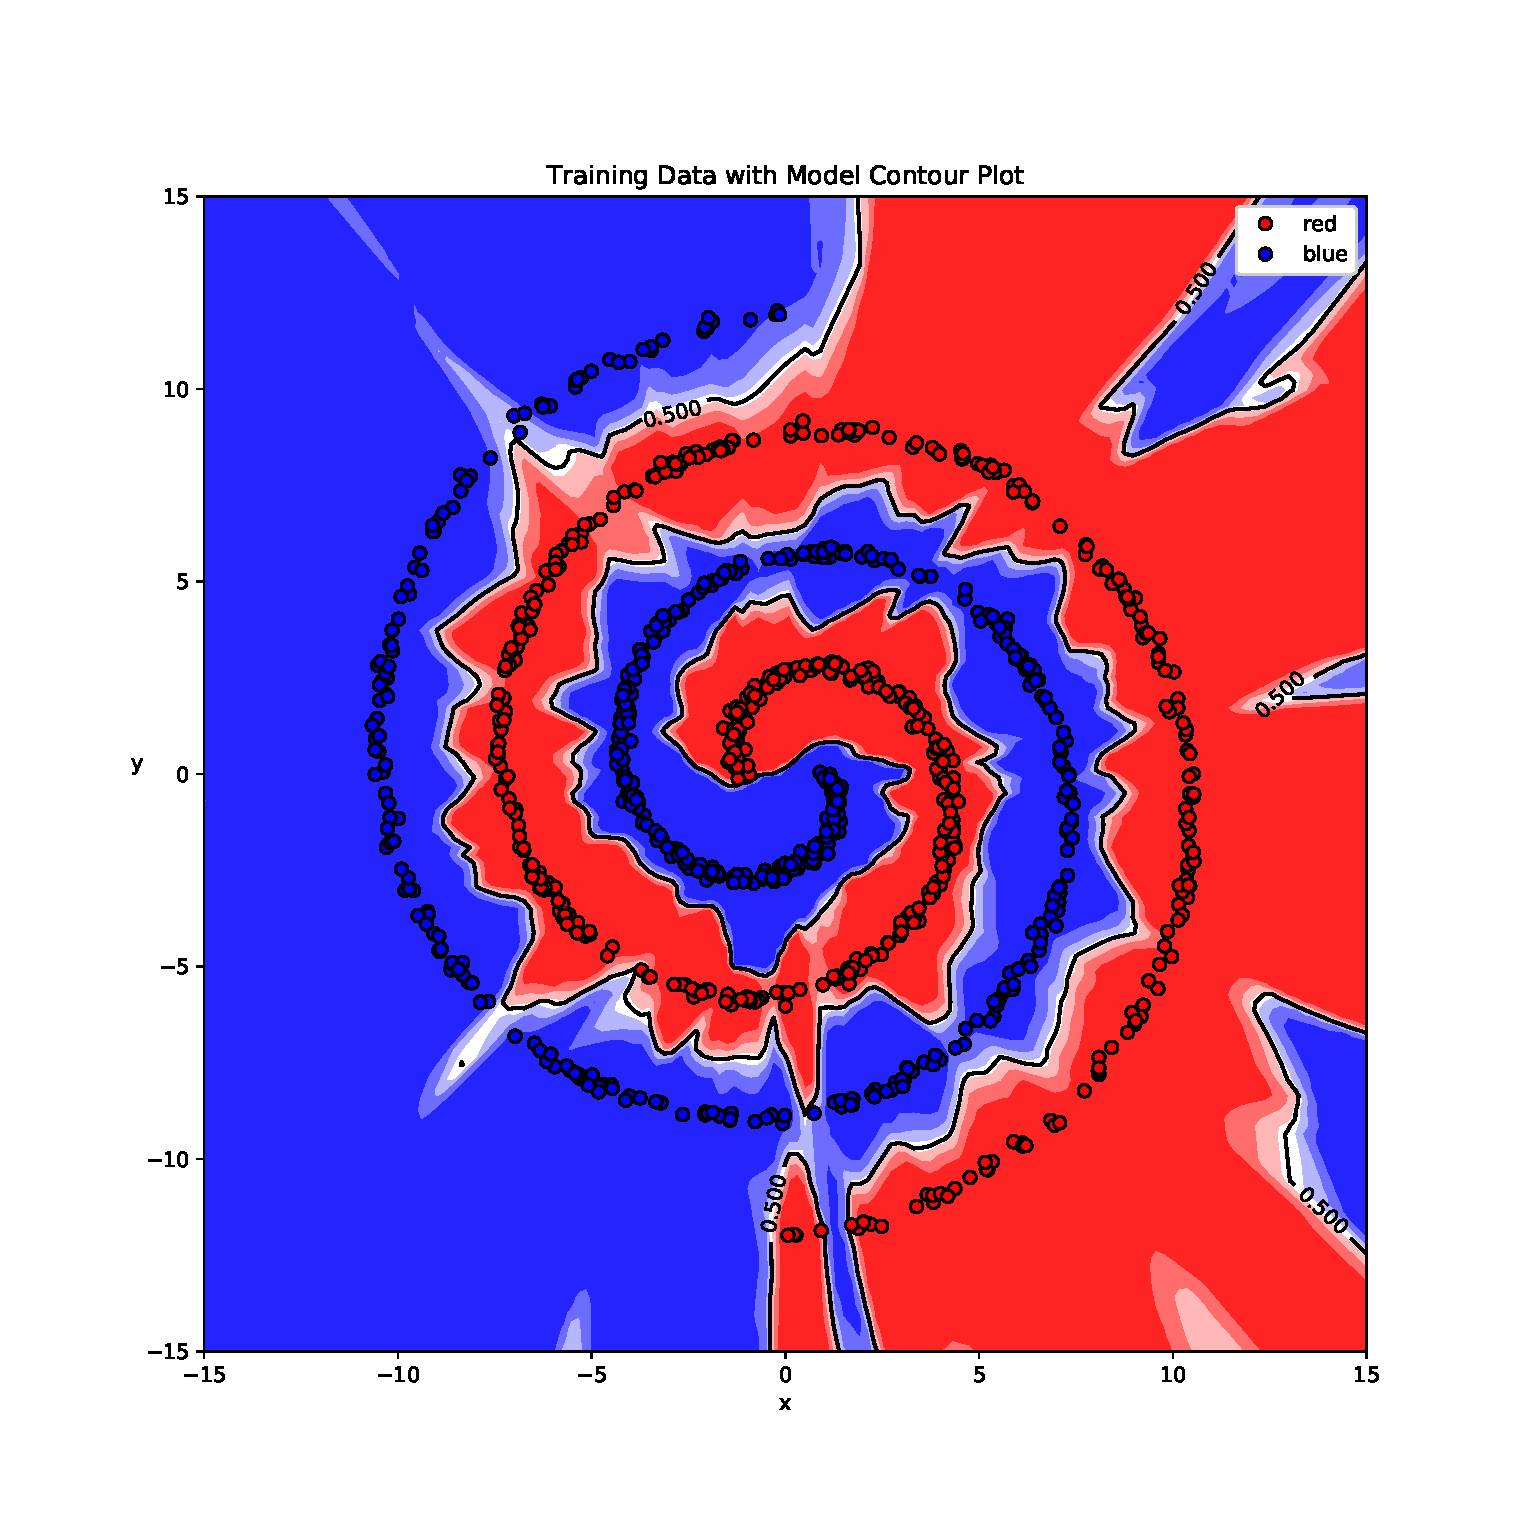
\includegraphics[width=0.75\textwidth]{Contour.eps}
   \caption{A plot of each of the basis functions, with the weights and intercept removed.}
\end{figure}

I knew from the beginning that I wanted to use a linear form for each layer (i.e. $\vec{w}^{T} \vec{x} + \vec{b}$) as discussed in class to keep the model simple, so the largest obstacle was determining which activation function to use. I originally implemented the sigmoid $\frac{1}{1 + e^{-x}}$ as a helper function and encountered problems where SGD couldn't calculate the gradient. Switching to \textit{tf.nn.sigmoid} resolve the problem, but in training the model seemed to learn incorrectly, classifying the entire left (along the x-axis) half of the points as red and the entire right half as blue. To correct this I switched to \textit{tf.nn.elu}, which yielded better, but still bad results. My model now uses \textit{tf.nn.relu6}, which yielded the best results through trial and error.

\clearpage
\begin{adjustwidth}{-50pt}{0pt}

\section{Code}

\begin{Verbatim}
import matplotlib as mpl
import matplotlib.pyplot as plt
import numpy as np
from numpy.linalg import norm
import tensorflow as tf

mpl.cm.register_cmap(cmap = mpl.cm.bwr_r)
NUM_SAMP = 512
NUM_SPIRALS = 1.75
NUM_BATCHES = 512
LEARNING_RATE = 0.1
BATCH_SIZE = 196
SIGMA_NOISE = .1
L2_PENALTY_SCALE = 0.2
np.random.seed(31415)
tf.random.set_seed(31415)
SCALE = 10

class Data(object):
   def __init__(self, num_samp = NUM_SAMP):
      
      # Equations to generate spirals
      theta = np.random.uniform(low = 0,
      high = (NUM_SPIRALS)*2*np.pi,
      size = (NUM_SAMP, 1))
      r = 1 + theta
      
      RED = 0
      BLUE = 1
      
      self.index = np.arange(NUM_SAMP*2)
      
      self.epsilon = np.random.normal(loc = 0,
      scale = SIGMA_NOISE,
      size = (4*NUM_SAMP, 1))
      
      x_red_epsilon = self.epsilon[:len(self.epsilon)//4]
      y_red_epsilon = self.epsilon[len(self.epsilon)//4:len(self.epsilon)//2]
      x_blue_epsilon = self.epsilon[len(self.epsilon)//2:3*len(self.epsilon)//4]
      y_blue_epsilon = self.epsilon[3*len(self.epsilon)//4:]
      
      self.x_red = -1*r*np.cos(theta) + x_red_epsilon
      self.y_red = r*np.sin(theta) + y_red_epsilon
      self.x_blue = r*np.cos(theta) + x_blue_epsilon
      self.y_blue = -1*r*np.sin(theta) + y_blue_epsilon
      
      self.red = np.concatenate([self.x_red, self.y_red], axis = 1)
      self.blue = np.concatenate([self.x_blue, self.y_blue], axis = 1)
      
      self.points = np.concatenate((self.red, self.blue), axis = 0)
      self.labels = np.array([RED] * (NUM_SAMP) + [BLUE] * (NUM_SAMP))

   def get_batch(self):
      """
      Select random subset of examples for training batch
      """
      
      choices = np.random.choice(self.index, size=BATCH_SIZE)
      
      batch_points = self.points[choices, :]
      batch_labels = self.labels[choices].flatten()
      return batch_points, batch_labels

class Model(tf.Module):
   def __init__(self):
      num_nodes_1 = 50
      num_nodes_2 = 50
      output_nodes = 1
      
      # Layer 1
      self.layer_1_weights = tf.Variable(
      		tf.random.normal(shape=[num_nodes_1, 2]))
      self.layer_1_bias = tf.Variable(tf.zeros(shape=[num_nodes_1, 1]))
      
      # Layer 2
      self.layer_2_weights = tf.Variable(
      		tf.random.normal(shape=[num_nodes_2, num_nodes_1]))
      self.layer_2_bias = tf.Variable(tf.zeros(shape=[num_nodes_2, 1]))
      
      # Layer 3
      self.layer_3_weights = tf.Variable(
      		tf.random.normal(shape=[output_nodes, num_nodes_2]))
      self.layer_3_bias = tf.Variable(tf.zeros(shape=[output_nodes, 1]))
      
      def __call__(self, points):
      layer_1_logits = self.layer_1_weights @ points.T + self.layer_1_bias
      output_1 = tf.nn.relu6(layer_1_logits)
      
      layer_2_logits = self.layer_2_weights @ output_1 + self.layer_2_bias
      output_2 = tf.nn.relu6(layer_2_logits)

      self.output_logits = tf.squeeze(self.layer_3_weights @ output_2 + self.layer_3_bias)
      return self.output_logits

   def compute_loss(self, labels):
      labels = list(map(float, labels))
      entropy = tf.reduce_mean(
     	 tf.nn.sigmoid_cross_entropy_with_logits(
	      logits = self.output_logits,
	      labels = labels)
	      )
      L2_PENALTY = L2_PENALTY_SCALE*(
         norm(tf.squeeze(model.layer_1_weights))**2
	     + norm(tf.squeeze(model.layer_2_weights))**2
	     + norm(tf.squeeze(model.layer_3_weights))**2
	     )
      loss = entropy + L2_PENALTY
      return loss

class Plotter:

   def __init__(self, data, model):
      self.data = data
      self.model = model

   def plot_original_data(self, filename = "Data.eps"):
      # Save original data
      plt.figure(figsize = (SCALE, SCALE))
      plt.scatter(self.data.x_red,self.data.y_red, c = "red", edgecolors = "black")
      plt.scatter(self.data.x_blue,self.data.y_blue, c = "blue", edgecolors = "black")
      plt.title("Raw Spiral Points")
      plt.xlabel('x')
      plt.ylabel('y',rotation=0)
      plt.savefig(filename)

   def plot_decision_boundary(self,
      	x_bound = [-15, 15], y_bound = [-15, 15],
      	filename = "Contour.eps"):
      NUM_POINTS = 150
      
      # Model the contour plot so we can see the decision boundary
      plt.figure(figsize = (SCALE, SCALE))
      plt.title("Training Data with Model Contour Plot")
      plt.xlabel('x')
      plt.ylabel('y',rotation=0)
      
      X, Y = np.meshgrid(
      	np.linspace(x_bound[0], x_bound[1], NUM_POINTS),
      	np.linspace(y_bound[0], y_bound[1], NUM_POINTS))
      Z = np.zeros((NUM_POINTS,NUM_POINTS))
      
      for i in range(NUM_POINTS):
      for j in range(NUM_POINTS):
      contour_points = np.array([ X[i,j], Y[i,j] ]).reshape(1,2)
      contour_logits = self.model(contour_points)
      Z[i,j] = tf.nn.sigmoid(contour_logits)
      
      plt.contourf(X, Y, Z, cmap = mpl.cm.bwr_r)
      
      plt.plot(self.data.x_red, self.data.y_red, 'or', markeredgecolor="black")
      plt.plot(self.data.x_blue, self.data.y_blue, 'ob', markeredgecolor="black")
      plt.legend(["red", "blue"])
      
      decision_boundary = plt.contour(X, Y, Z, levels = [0.5], colors = "black")
      plt.clabel(decision_boundary, colors='black')
      
      plt.savefig(filename)

if __name__ == "__main__":
   data = Data()
   model = Model()
   optimizer = tf.optimizers.SGD(learning_rate=LEARNING_RATE)
   bar = range(NUM_BATCHES)
   for i in bar:
      with tf.GradientTape() as tape:
         points, labels = data.get_batch()
         logits = model(points)
         loss = model.compute_loss(labels)
         grads = tape.gradient(loss, model.variables)
         optimizer.apply_gradients(zip(grads, model.variables))
   
   plotter = Plotter(data, model)
   plotter.plot_original_data()
   plotter.plot_decision_boundary()
\end{Verbatim}
\end{adjustwidth}

\end{document}